\documentclass[tikz]{standalone}
\usepackage{pgfplots}
%\pgfplotsset{width=7cm,compat=1.18}
\usepgfplotslibrary{statistics}
\def\axisdefaultwidth{6cm}
\def\axisdefaultheight{6cm}
%\pgfplotsset{every axis/.style={scale only axis}} 		

\begin{document}
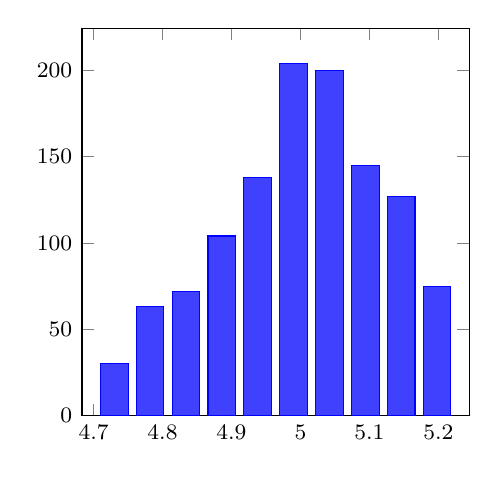
\begin{tikzpicture}
%\begin{axis}[small,ymin=0,title=\texttt{vcmmax}]
\begin{axis}[small,ymin=0]
\addplot [
ybar,
fill=blue!75,
draw=blue]
table [x=perf, y=cnt] {
cnt                 perf                
30.00000            4.73001             
63.00000            4.78201             
72.00000            4.83401             
104.00000           4.88601             
138.00000           4.93801             
204.00000           4.99001             
200.00000           5.04200             
145.00000           5.09400             
127.00000           5.14600             
75.00000            5.19800             
};
\end{axis}
\end{tikzpicture}
\end{document}
